% ProductieTechnologie-Samenvatting-RubenRyckaert.tex
% Simple layout template with helpers for chapters, a formularium, and an easy figure helper.

\documentclass[a4paper,12pt,twoside]{report}
\usepackage[utf8]{inputenc}
\usepackage[dutch]{babel}
\usepackage[T1]{fontenc}
% Use default (Computer Modern) but ensure scalable fonts via Latin Modern, keep microtype
\usepackage{lmodern}
\usepackage[activate={true,nocompatibility},final,tracking=true,kerning=true,spacing=true,stretch=10,shrink=10]{microtype}
% Ensure microtype uses the correct spacing model with nonfrenchspacing
\microtypecontext{spacing=nonfrench}
% Slightly increase line spacing for readability
\usepackage{setspace}
\setstretch{1.15} % slightly larger for better readability on A4
% Make TeX less strict about individual line breaks to reduce underfull boxes
\sloppy
\usepackage{amsmath,amssymb}
\usepackage{graphicx}
\usepackage{tikz}
% TikZ libraries used by figures (calc for coordinate arithmetic, arrows.meta for arrow tips, positioning for nodes)
\usetikzlibrary{calc,arrows.meta,positioning}
\usepackage{fancyhdr}
\usepackage{tcolorbox}
\usepackage{float}
% Page geometry: reduce margins and make them consistent
\usepackage[left=2.0cm,right=2.0cm,top=2.5cm,bottom=2.5cm]{geometry}
% Configure hyperref to avoid duplicate destination names (see hyperref option `hypertexnames`)
\usepackage[hidelinks,hypertexnames=false]{hyperref}
% Use `bookmark` to make outline writing more robust and avoid "file has changed" rerun warnings
\usepackage{bookmark}
\usepackage{caption}
\captionsetup{skip=3pt,aboveskip=3pt,belowskip=3pt} % reduce caption separation
\usepackage{enumitem}% Shared project macros (\frm, formularium, \fig)
\usepackage{./productie-macros}

% --- Practical packages & macros to improve writing and consistency ---
% Units & numbers (guarded: compiles even if siunitx is not installed)
\IfFileExists{siunitx.sty}{%
  \usepackage{siunitx}%
  \sisetup{per-mode=symbol,detect-all=true}%
}{%
  \PackageWarning{productie-macros}{Package `siunitx' not found; install it to enable \string\SI and unit formatting (tlmgr install siunitx)}%
}
% Better tables
\usepackage{booktabs}
% Sub-figures
\usepackage{subcaption}
% Smart cross-references (load after hyperref) — guarded so missing package doesn't break build
\IfFileExists{cleveref.sty}{%
  \usepackage[capitalise]{cleveref}%
  % Localised names (Dutch)
  \crefname{figure}{figuur}{figuren}
  \Crefname{figure}{Figuur}{Figuur}
  \crefname{table}{tabel}{tabellen}
  \Crefname{table}{Tabel}{Tabel}
}{%
  \PackageWarning{productie-macros}{Package `cleveref' not found; use standard \ref for cross-references}%
}

% Handy short macros for frequently used symbols
\newcommand{\Fc}{\ensuremath{F_c}}
\newcommand{\vc}{\ensuremath{v_c}}
\newcommand{\Pc}{\ensuremath{P_c}}

% Small helper for quick theory/exercise inline boxes (uses tcolorbox loaded earlier)
\newtcbox{\theoriebox}{on line,boxrule=0.4pt,arc=2pt,boxsep=3pt,top=2pt,bottom=2pt,colback=gray!6,colframe=gray!40}

% Quick usage notes:
% - Use \SI{120}{\milli\metre\per\minute} for units (siunitx)
% - Use \cref{fig:label} for cross-references (cleveref)
% - Use \toprule/\midrule/\bottomrule for nicer tables (booktabs)

% Hyphenation & tolerance adjustments to reduce underfull boxes
% Increase tolerance slightly and give TeX more emergency stretch so fewer
% underfull \hbox warnings occur in compact technical text
\tolerance=1000
\hyphenpenalty=300
\exhyphenpenalty=300
\emergencystretch=2em
% If you see a Babel warning about Dutch hyphenation patterns, install them
% and rebuild your format (tlmgr or system package manager) to enable real
% Dutch hyphenation and reduce badness further
\AtBeginDocument{\PackageWarning{productie-macros}{If you see ``No hyphenation patterns were preloaded for the language "Dutch"'' please install Dutch hyphenation patterns and rebuild your TeX format (e.g., using tlmgr).}}

% Allow ragged bottom so LaTeX doesn't stretch pages to fill vertical space
\raggedbottom
% For customizing chapter styles and safely patching \chapter
\usepackage{etoolbox}
\usepackage{titlesec}
% Prevent figures from floating past chapter boundaries and ensure floats don't appear before they are defined
\usepackage{placeins}
\usepackage{flafter}
% Insert a FloatBarrier before every \chapter to keep floats in their chapter
\preto\chapter{\FloatBarrier}

% Make chapters keep number and title on the same line and avoid forcing a new page
\makeatletter
\patchcmd{\chapter}{\if@openright\cleardoublepage\else\clearpage\fi}{}{}{}
\makeatother
% Slightly smaller chapter titles (keep them prominent but less tall)
\titleformat{\chapter}[hang]{\normalfont\LARGE\bfseries}{\thechapter}{1em}{}
\titlespacing*{\chapter}{0pt}{12pt}{6pt} % more breathing room before/after chapter titles
% Ensure section and subsection align to same left margin and use sensible spacing
% Slightly reduce section/subsection size so titles are less dominant
\titleformat{\section}[hang]{\normalfont\large\bfseries\raggedright}{\thesection}{1em}{}
\titlespacing*{\section}{0pt}{10pt}{6pt} % increase space before/after section titles
\titleformat{\subsection}[hang]{\normalfont\normalsize\bfseries\raggedright}{\thesubsection}{1em}{}
\titlespacing*{\subsection}{0pt}{8pt}{4pt} % increase space for subsections

% Paragraph spacing and list defaults for consistent left alignment
\setlength{\parindent}{0pt} % if you prefer paragraph indent restore this to 1em
\setlength{\parskip}{0.6ex plus 0.15ex} % increase parskip slightly for better readability
% Compact list indentation (smaller distance from page margin)
% Increase vertical spacing and indent lists slightly for readability
% Tweak: larger topsep/partopsep for space before/after list; small itemsep between items; larger left margins
\setlist[itemize,1]{leftmargin=1.6em,itemsep=0.35ex,parsep=0.2ex,partopsep=0.4ex,topsep=0.6ex}
\setlist[itemize,2]{leftmargin=2.2em,itemsep=0.25ex,parsep=0.15ex,partopsep=0.3ex,topsep=0.45ex}
\setlist[enumerate,1]{leftmargin=1.6em,itemsep=0.35ex,parsep=0.2ex,partopsep=0.4ex,topsep=0.6ex}
\setlist[enumerate,2]{leftmargin=2.2em,itemsep=0.25ex,parsep=0.15ex,partopsep=0.3ex,topsep=0.45ex}
% ------------------ Header / Footer ------------------
% Avoid fancyhdr warning about small headheight
\setlength{\headheight}{14pt}
\pagestyle{fancy}
\fancyhf{}
\fancyhead[LE,RO]{\small\bfseries\thepage}
\fancyhead[LO,RE]{\small\nouppercase{\leftmark}}
\renewcommand{\headrulewidth}{0.3pt}
% Reduce vertical spacing around floats to avoid large gaps
\setlength{\floatsep}{6pt plus 1pt minus 1pt}     % between floats
\setlength{\textfloatsep}{8pt plus 1pt minus 1pt} % between floats and text
\setlength{\intextsep}{6pt plus 1pt minus 1pt}    % for in-text floats (top/bottom of figure)

% ------------------ Formularium helpers ------------------
% Provided by `productie-macros.sty` (\frm, formularium, \fig helpers).  
% You can override box colors using \setfrmcolors{<back>}{<frame>} after loading the package.

% ------------------ Figure helper ------------------
% Provided by `productie-macros.sty` via the \fig helper.
% Provide a small, non-invasive fallback for \autofig (used in some places).
% This uses \providecommand so it will only define \autofig when it isn't
% already defined by `productie-macros.sty`.
\providecommand{\autofig}[3][]{%
  \begin{figure}[ht]
    \centering
    \includegraphics[#1]{#2}
    \caption{#3}
  \end{figure}
}

% ------------------ Document metadata ------------------
\title{Productietechnologie — Samenvatting}
\author{Ruben Ryckaert}
\date{\today}

\begin{document}
\maketitle
\microtypesetup{protrusion=false}
% Also disable protrusion for LoF and LoT so those lists use consistent spacing
\pretocmd{\listoffigures}{\microtypesetup{protrusion=false}}{}{}
\apptocmd{\listoffigures}{\microtypesetup{protrusion=true}}{}{}
\pretocmd{\listoftables}{\microtypesetup{protrusion=false}}{}{}
\apptocmd{\listoftables}{\microtypesetup{protrusion=true}}{}{}
\tableofcontents
\microtypesetup{protrusion=true}

\begin{formularium}
% Formularium entries can be added here if needed
\end{formularium}


\chapter{Inleiding}
\textbf{Wat is Productietechnologie?}

Productietechnologie gaat over het produceren van goederen. Hier komt veel bij te pas: niet alleen verschillende technieken en machines, maar ook kosten, snelheid en kwaliteit spelen een rol.

Deze samenvatting geeft een overzicht van de belangrijkste begrippen en technieken.


\textbf{Hieronder verschillende productietechnieken,}
\begin{itemize}
  \item Gieten
    \begin{itemize}
      \item Zandgieten
      \item Spuitgieten
    \end{itemize}
  \item Frezen
  \item Lassen
    \begin{itemize}
      \item CO2-lassen
      \item MIG/MAG, TIG, \ldots
    \end{itemize}
  \item Vonkerosie
  \item Waterstraalsnijden
  \item Chemisch bewerken
  \item 3D-printen
  \item Draaien
  \item Snijden
  \item Ponsen
  \item Stralen
  \begin{figure}[ht]
  \centering\includegraphics[width=0.5\textwidth]{straalbewerkingen.png}
  \caption{Overzicht van bewerkingen met stralen, gebruikmakend van verschillende energiedragers}
  \label{fig:stralen_overzicht}
\end{figure}
\end{itemize}

\subsection{Keuzes bij productie}

Bij produceren moet je afhankelijk van al deze technieken
keuzes maken over welke technieken het beste is. Hoeveel producten
moet ik produceren en wat kost dat? Het is allemaal afhankelijk 
van de eisen die aan het product worden gesteld.

\begin{itemize}
  \item Kosten
  \item snelheid
  \item kwaliteit
  \item milieu
  \item veiligheid
  \item functionaliteit
  \item materiaal
  \item tolerantie
  \item oppervlaktekwaliteit
  \item aantal
  \item onderhoud
\end{itemize}

al deze factoren zijn belangrijk bij het kiezen van een productietechniek.


\section{Passing}

Passing is een maat voor hoe goed twee oppervlakken op
 elkaar aansluiten.

 \begin{itemize}
    \item Losse Passing: Er is nog speling tussen de twee oppervlakken.
    \item Nauw Passing: De twee oppervlakken sluiten goed op elkaar aan, er is
      bijna geen speling meer.
    \item PersPassing: De twee oppervlakken worden in elkaar gedrukt.
 \end{itemize}

 \section{Tolerantie}
    Toleranties worden geklassificeerd via diagrammen 

    \begin{itemize}
        \item inwendige
        \item uitwendige
        \item passing 
    \end{itemize}

    \begin{figure}[ht]
      \centering
      \includegraphics[width=0.32\textwidth]{image1.png}\hfill
      \includegraphics[width=0.32\textwidth]{image2.png}\hfill
      \includegraphics[width=0.32\textwidth]{image3.png}
      \caption{Tolerantie diagrammen voor inwendige, uitwendige en passing}
      \label{fig:tolerantie_diagrammen}
    \end{figure}

    Je moet kiezen welke tolerantie nodig is voor een product.
    Precieze toleranties zijn duurder om te produceren.

    \begin{figure}[ht]
      \centering
      \includegraphics[width=0.5\textwidth]{image5.png}
      \caption{Kosten vs Tolerantie}
      \label{fig:kosten_vs_tolerantie}
    \end{figure}

    \section{Oppervlaktekwaliteit}
    Oppervlaktekwaliteit moet ook gekozen worden bij het produceren van een product.
    \begin{itemize}
      \item Een ruw oppervlak is goedkoper om te produceren.
      \item Een glad oppervlak is duurder om te produceren.
      \item Soms is een glad oppervlak nodig voor de functionaliteit van het product.
      \item Textuur kan ook functioneel zijn (antislip, esthetisch, \ldots). bv: een
        handvat, keyboard, tafels, pennen, \ldots
    \end{itemize}

    Oppervlaktekwaliteit wordt uitgedrukt in ruwheid.
    Ra, Rz, Rmax

\begin{figure}[ht]
  \centering
  \includegraphics[width=0.4\textwidth]{image6.png}\hfill
  \includegraphics[width=0.4\textwidth]{image7.png}
  \caption{Voorbeelden van oppervlaktekwaliteiten}
  \label{fig:oppervlaktekwaliteiten}
\end{figure}

  verschillende productietechnieken hebben verschillende oppervlaktekwaliteiten.



  \chapter{Materialen}

  Dit hoofdstuk gaat over de effecten van verschillende materialen op productietechnieken en over het effect van de gekozen productietechniek op het materiaal.

  \begin{figure}[ht]
  \centering
  \includegraphics[width=0.5\textwidth]{image9.png}
  \caption{Effect van thermische process op materialen}
  \label{fig:image9}
\end{figure}

  Er zijn verschillende soorten materialen die je kunt kiezen.
  Allemaal hebben ze verschillende materiaaleigenschappen.
  \begin{itemize}
    \item Metalen
    \item Kunststoffen
    \item Keramiek
    \item Composieten
  \end{itemize}

  \subsection{Vervorming}

  Je hebt elastische en plastische vervormingen in een materiaal die gebeureren
  tijden het bewerken van een materiaal.
  \begin{itemize}
    \item Elastische vervorming: Het materiaal keert terug naar zijn originele vorm
      nadat de kracht is weggenomen.
    \item Plastische vervorming: Het materiaal blijft vervormd nadat de kracht is
      weggenomen.
  \end{itemize}
  Elastische vervorming gegeven door Hooke's law:
  \frm{Hooke's law}{\sigma = E \cdot \varepsilon}{waarbij $\sigma$ de spanning is, $E$ de elasticiteitsmodulus en $\varepsilon$ de rek.}


\chapter{Verspanen:Algemeen}
\label{chap:Algemeen verspanen}
\textbf{Dit hoofdstuk is de basis van verspannen en is relevant voor alle verspaningstechnieken.}

  Verspannen is het verwijderen van materiaal van een werkstuk. Dit kan door boren, frezen, draaien of slijpen, \ldots Je begint met een ruw werkstuk en verwijdert materiaal totdat je de gewenste vorm en afmetingen hebt.



  \textbf{Voordelen}
  \begin{itemize}
    \item Hoge precisie
    \item Goede tolerantie
    \item Goede oppervlaktekwaliteit
    \item Flexibiliteit in ontwerp
  \end{itemize}

  \textbf{Nadelen}
  \begin{itemize}
    \item Materiaalverlies
    \item Hogere kosten bij grote aantallen
    \item Langere productietijd
    \item energieintensies
    \item Vervuilend (spanen, koelvloeistof)
  \end{itemize}

  Bij verspannen kunnen verschillende tools gebruikt worden.
  Deze tools hebben verschillende snijvlakken en geometrieën
  die geschikt zijn voor verschillende materialen en bewerkingen.

  \begin{itemize}
    \item bijtel
    \item frees
    \item boor
    \item slijpschijf
  \end{itemize}

  \section{bijtelbewerkingen}

  Bij bijtelbewerkingen wordt materiaal verwijderd door een scherpe
  bijtel over het werkstuk te bewegen.
  \begin{figure}[H]
  \centering
  \includegraphics[width=0.6\textwidth]{image10.png}
  \caption{Verwijdering van materiaal door een bijtel $\to$ creëert spanen}
  \label{fig:image10}
\end{figure}

  Bij het verspannen met een bijtel ontstaan er spanen.
  Spanen zijn kleine stukjes materiaal die worden verwijderd
  van het werkstuk.
  De grootte van de spanen wordt bepaald door de snedediepte, de voeding, de spaanhoek en de wrijvingscoëfficiënt.\ldots Zometeen meer in detail hierover

  Spanen is een plastische vervorming van de spanen
  maar het oppervlak van het werkstuk ondergaat ook een elastische vervorming.
  Dit kan leiden tot oppervlaktefouten zoals ruwheid, hardheid, \ldots




\begin{figure}[ht]
  \centering
  \includegraphics[width=0.8\textwidth]{image11.png}
  \caption{}
  \label{fig:image11}
\end{figure}

\frm{Afschuifhoek}{\phi = 45^{\circ} + \dfrac{\gamma}{2} - \dfrac{\mu}{2}}{waarbij $\gamma$ de spaanhoek is en $\mu$ de wrijvingshoek tussen spaan en snijvlak.}

De afschuifhoek bepaalt de richting waarin de spaan wordt afgesneden.
Een grotere afschuifhoek leidt tot een betere spaanvorming en minder kracht

\frm{afschuifvlak (shear zone) A}{A = \frac{b*h}{\sin(\phi)}}{waarbij $b$ de breedte, $h$ de hoogte en $\phi$ de afschuifhoek.}
\begin{figure}[ht]
  \centering
  \includegraphics[width=0.4\textwidth]{image20.png}
  \caption{}
  \label{fig:image20}
\end{figure}

\frm{afschuifkracht}{F = A*\tau}{waarbij $A$ het afschuifvlak is en $\tau$ de schuifspanning van het materiaal.}

Grotere spaanhoek $\to$ kleiner afschuifvlak $\to$ minder kracht nodig om spaan te vormen.


\subsection{Secundaire afschuifvlak(shear zone)}
Spanen gaan verwijderd worden en daarbij treedt wrijving op tussen spaan en bijtel; dit is het secundaire afschuifvlak. Als je negatieve spaanhoeken $\gamma$ meet, dan is er veel meer wrijving tussen de spaan en de bijtel.

\begin{itemize}
  \item Spaanhoek $\gamma$ $\to$ groter $\to$ minder kracht nodig. Tussen -10° en 30°
  \item Wighoek $\beta$ $\to$ zo groot mogelijk maken.
  \subitem Wighoeken bepalen de sterkte van de bijtel en de warmteafvoer. Grote wighoeken brengen de warmte sneller weg
  en dus kun je grotere voedingsnelheden gebruiken.
  \subitem Wighoek moet zo groot mogelijk zijn
    \begin{figure}[ht]
    \centering
    \includegraphics[width=0.4\textwidth]{image12.png}
    \caption{Wighoek}
    \label{fig:image12}
  \end{figure}
  \item Vrijloophoek $\alpha$ $\to$ groter $\to$ minder wrijving tussen werkstuk en bijtel. Tussen 6° en 10°
  \subitem Vrijloophoek moet er zijn zodat je bijtel niet begint te wrijven over het oppervlakte van je materiaal.
  Zelfs rond 0° kan al zorgen voor veel wrijving.
    \begin{figure}[ht]
    \centering
    \includegraphics[width=0.4\textwidth]{image14.png}
    \caption{Vrijloophoek}
    \label{fig:image14}
  \end{figure}
  \item Snedediepte $\to$ groter $\to$ meer kracht nodig
  \item Voeding $\to$ groter $\to$ meer kracht nodig
\end{itemize}

Deze verschillende hoeken hebben effect op elkaar. Dit is dus een optimalisatieprobleem. Je moet afwegen wat de beste hoeken zijn voor jouw materiaal en bewerking.

De spaanhoek is enorm belangrijk. Een grote spaanhoek snijdt makkelijk
materialen zoals aluminium, koper, kunststof.
Voor hardere materialen zoals staal is een kleinere spaanhoek nodig
omdat het materiaal anders te hard is om te snijden en je moet veel te veel kracht zetten.
Negatieve spaanhoeken worden gebruikt voor zeer harde materialen.

\subsubsection{Extra info}
Deze bewerkingen zijn allemaal met ductiele materialen. 
Brosse materialen gaan snel afbrokkelen en hebben dus niet veel elastische vervorming. Je kunt druk uitoefenen op brosse materialen tijdens bewerking; het materiaal gaat zich dan meer ductiel gedragen.
 Hoe oefen je druk uit op materialen? Door een grote spaanhoek te gebruiken,
  die veel spanning creëert.



\begin{figure}[ht]
  \centering
  \includegraphics[width=0.5\textwidth]{image15.png}
  \caption{Verschillende spaanhoeken voor verschillende materialen}
  \label{fig:image15}
\end{figure}



\section{Beweging, snelheden en voedingen, temperaturen, slijtage}

Er zijn verschillende factoren die de kracht op je werkstuk bepalen
\begin{itemize}
  \item Snijsnelheid (v)
  \item Voeding (f)
  \item Snedediepte (a)
  \item Snedebreedte (b)
  \item Snededikte (h)
\end{itemize}

\frm{Snijsnelheid}{v = \pi \cdot d \cdot n}{waarbij $d$ de diameter is en $n$ het toerental in omwentelingen per minuut.}

\begin{figure}[ht]
  \centering
  \includegraphics[width=0.4\textwidth]{image16.png}
  \caption{Snededoorsnede bij bijtelbewerking}
  \label{fig:image16}
\end{figure}

\frm{Snededoorsnede}{A_d = a \cdot b}{waarbij $a$ de snedediepte is en $b$ de snedebreedte.}


\subsection{Krachten}
Tijdens het bewerken van materialen met een bijtel
komen er verschillende krachten op het werkstuk en de bijtel te staan.

\begin{itemize}
  \item Snijkracht (Fc): Kracht die nodig is om de spaan te vormen.
  \item Voedingskracht (Ff): Kracht die in de voedingsrichting werkt.
  \item Terugdrukkracht (Fp): Kracht die nodig is om de bijtel in het werkstuk te duwen.
  \begin{figure}[ht]
  \centering
  \includegraphics[width=0.4\textwidth]{image17.png}
  \caption{}
  \label{fig:image17}
\end{figure}

\end{itemize}

\textbf{Wat neem voeding op?}
\begin{itemize}
  \item Warmteontwikkeling
  \item Werkstuk
  \item Gereedschap
  \item Spaanvorming
  Afhankelijk van de snijsnelheid $v_c$ en de voeding $f$. is er een andere verdeling van de energie.
  \begin{figure}[ht]
    \centering
    \includegraphics[width=0.4\textwidth]{image21.png}
    \caption{Voeding of snijsnelheid in functie van energieverdeling}
\end{figure}
\end{itemize}

\section{Factoren bij bijtelbewerking}
\begin{itemize}
  \item \textbf{Opbouwlaag (build-up edge/BUE)}

    Een dunne, hard geworden laag metaal die 
        zich bij lage snijsnelheden aan het snijgereedschap 
        opbouwt aan de punt van de bijtel. Zie video toledo.  
        Deze stukken trekken mee aan het oppervlak van het werkstuk en nemen dus meer af dan nodig is.
        Je krijgt dan een stappige oppervlakte.

        \paragraph{Verbeteren / voorkomen:}
        \begin{itemize}
          \item Verhoog de snijsnelheid: bij hogere snelheden herstelt het materiaal sneller, waardoor BUE minder snel vormt.
          \item Gebruik koeling of smering: vermindert hechten en verlaagt gereedschapstemperatuur.
          \item Kies geschikte gereedschapsmaterialen en coatings (bv. TiN/AlTiN) en houd de snijkant scherp.
          \item Pas voeding en snedediepte aan of gebruik onderbroken snedes (pecking) om opbouw te vermijden.
          \item Controleer en vervang gereedschap regelmatig; verwijder opbouwranden veilig indien nodig.
        \end{itemize}

    



  \item \textbf{Warmte}

    Deze processen genereren veel warmte. Dit kan het materiaal aan de oppervlakte
    vervormen, leiden tot veranderde hardheid en ruwheid en verhoogde slijtage.
    Er zijn verschillende manieren om de warmte te verminderen:
    \begin{itemize}
      \item Koelen met koelvloeistof -> hoge nauwkeurigheid en lage ruwheid.
      \item Smeren met olie -> hogere snijsnelheid mogelijk, hogere voeding.
      \item Spaanafvoer optimaliseren -> vermijd ophoping van spanen die warmte vasthouden.
      \item Werkstuk emulseren in water, koelvloeistof of olie.
    \end{itemize}

    Warmte wordt op het werkstuk op drie plaatsen gecreeerd:
    1. Afschuifvlak (shear zone):
    2. Secundaire afschuifvlak (tussen spaan en bijtel):
    3. Vrijloopvlak (tussen werkstuk en bijtel): 

    \begin{figure}[ht]
      \centering
      \includegraphics[width=0.7\textwidth]{image18.png}
      \caption{}
    \end{figure}

  \item \textbf{Spaanvorming}

    Spanen kunnen het werkstuk beschadigen als ze niet goed worden afgevoerd.
    Dit kan leiden tot krassen en ruwheid.
    \begin{itemize}
      \item Continue spaanvorming
      \item Lamelsspaan
      \item brokspaan
    \end{itemize}

  \item \textbf{Slijtage}

    Tijdens het bewerken van materialen slijt het gereedschap.
    Dit kan leiden tot een slechtere oppervlaktekwaliteit, hogere krachten,
    hogere temperaturen, enz.
    Slijtage kan veroorzaakt worden door:
    \begin{itemize}
      \item Vrijloopslijtage: door wrijving tussen gereedschap en werkstuk.
      \item Thermische slijtage: door hoge temperaturen die het gereedschap verzwakken
      \item Kerfslijtage: door herhaalde spanningsconcentraties bij het vrlijloopvlak.
      \item Breuk: Afbreken van een stuk
      \item Werkstukslijtage: Vlijloopvlak slijtage verhoogd met verbruik van de bijtel.
      \item Neusslijtage: slijtage aan de punt van de bijtel door hoge krachten en temperaturen.
    \end{itemize}

    \autofig[0.5\textwidth]{image23.png}{}

    Je kunt slijtage verminderen door:
    \begin{itemize}
      \item Gebruik van coatings op gereedschap (bv. TiN, AlTiN) om wrijving en hitte te verminderen.
      \item Optimaliseren van snijsnelheid, voeding en snedediepte om overmatige hitte en krachten te vermijden.
      \item Toepassen van koeling en smering om hitte af te voeren en wrijving te verminderen.
      \item Tool met lood PB gebruiken
        % use the \autofig helper to paste images safely; it auto-generates a sanitized label
        \autofig[0.5\textwidth]{image22.png}{}
        lood geeft minder slijtage omdat het smerende eigenschappen heeft -> minder wrijving.
\end{itemize}




\end{itemize}

\section{Snijmaterialen}
Met welk materiaal ga je je bijtel maken?
Je beitel moet ductiel zijn en taai zijn. Het perfecte gereedschap is goedkoop, ductiel en taai.

\begin{figure}
  \centering
  \includegraphics[width=0.5\textwidth]{image24.png}
  \caption{Relatieve hardheid in functie van temperatuur voor verschillende snijmaterialen}
\end{figure}


\begin{enumerate}
  \item \textbf{Snelstaal (HSS)( $v_c$ 6-12m/min).}
  gehard staal; geschikt voor algemene toepassingen bij lage tot matige snijsnelheden.
  Goedkoop om te maken.
  \item \textbf{Hardmetaal (wolframcarbide, WC + Co)} 
  hittebestendig; geschikt voor hogere snijsnelheden en hardere materialen dan HSS.
  \item \textbf{Gecoate hardmetaal ($v_c$ 60--600 m/min)}
    Dunne coatings (bv. TiN, AlTiN) verbeteren slijtvastheid en hittebestendigheid; de bovenste laag moet slijtage weerstaan terwijl binnenste lagen warmte afvoeren.
    \textbf{Productie:} PVD (Physical Vapor Deposition) of CVD (Chemical Vapor Deposition).
  
  \item \textbf{Keramiek in metaalmatrix (hoge $v_c$)}
    Zeer hard en hittebestendig; geschikt voor hoge snijsnelheden bij harde materialen. Keramische deeltjes zijn ingebed in een metaalmatrix (nitriden, oxiden of carbiden). Vermijd onderbroken sneden omdat keramiek bros is; houd de snijdedoorsnede klein.
  \item \textbf{Diamant} — zeer hard; beperkt toepasbaar bij bewerking van staal omdat diamant
   bij hoge temperaturen en in aanwezigheid van ijzer kan reageren en degraderen.
\end{enumerate}
Snelstaal is goedkoop, maar het wordt duurder naarmate je betere materialen gebruikt. Je moet dus bepalen hoe goed je gereedschap moet zijn voor jouw toepassing.

\begin{figure}[ht]
  \centering
  \includegraphics[width=0.6\textwidth]{image25.png}
  \caption{Overzicht van snijmaterialen en hun toepassingsgebieden}
\end{figure}
Al deze snijmaterialen zijn gecreeerd door de jaren heen.
Er wordt nog steeds onderzoek gedaan aan betere, goedkopere en duurzamere materialen. 


\subsection{Classificatie van snijmaterialen}


\begin{figure}[ht]
  \centering
  \includegraphics[width=1\textwidth]{image26.png}
  \caption{Classificatie van snijmaterialen}
\end{figure}

\textbf{belangrijk voor tijdens het examen. Hij kan een klasse gegeven
zoals in de figuur en jij moet weten waar dat voor staat!}

\section{Optimale snijsnelheid}

Bij alle machines worden inserts gebruikt voor bijtels. 
Als bijtels kapot gaan door slijtage, kan je die vervangen.
Je moet dus de optimale snijsnelheid kiezen
zodat je zo lang mogelijk met een insert kan werken

\begin{figure}[ht]
  \centering
  \includegraphics[width=0.5\textwidth]{image27.png}
  \caption{Klemming van Inserts in een houder}
\end{figure}

Bij grotere snijsnelheden is er meer slijtage.

\textbf{Je kunt de levensduur van een gereedschap voorspellen met de formule van Taylor:}
\frm{formule van Taylor}{v_c\, T^n = C}{waarbij $C$ een constante is en $n$ een materiaalconstante, $T$ de gereedschaplevensduur in minuten en $v_c$ de snijsnelheid in m/min.}

  Je kunt deze formule gebruiken om de optimale snijsnelheid te bepalen.

Hier zijn $C$ en $n$ materiaalconstanten. Deze formule laat zien hoe veranderingen in snijsnelheid de levensduur beïnvloeden.

Voorbeeld:

Gegeven: $n = 0.125$. Verhoog de snijsnelheid met $50\%$: $v_2 = 1.5\,v_1$.

Volgens Taylor: $v_1\,T_1^n = C$ en $v_2\,T_2^n = C$.
Daarom
\[
\frac{v_2}{v_1} = \left(\frac{T_1}{T_2}\right)^n
\]
en dus
\[
\frac{T_2}{T_1} = \left(\frac{v_2}{v_1}\right)^{-1/n} = (1.5)^{-1/0.125} = (1.5)^{-8} \approx 0.039.
\]
Dus als je de snijsnelheid met $50\%$ verhoogt, wordt de gereedschaplevensduur ongeveer $0.039$ keer zo groot — oftewel ongeveer $25$ keer korter.

De vraag is wat de optimale snijsnelheid is?
    

\begin{figure}[ht]
    \centering
    \includegraphics[width=0.8\textwidth]{image28.png}
    \caption{}
\end{figure}


\chapter{Verspanen: Draaien}
  Draaien is een veelgebruikte verspaningstechniek waarbij een roterend werkstuk
  wordt bewerkt met een bijtel om materiaal te verwijderen en de gewenste vorm te creëren.

  Je kunt hier verschillende bewerkingen mee uitvoeren:
  \begin{enumerate}
    \item \textbf{Langsdraaien}: Het verwijderen van materiaal langs de lengteas van het werkstuk om de diameter te verkleinen.
    \item \textbf{Vlakdraaien}: Het creëren van een vlak oppervlak aan het uiteinde van het werkstuk.
    \item \textbf{Insteekdraaien}: Het snijden van een groef of het afkappen van een deel van het werkstuk.
    \item \textbf{Schroefdraad Snijden}: Het creëren van schroefdraad op het oppervlak van het werkstuk.
\end{enumerate}

\textbf{Extra's:}

\textbf{Kopsteken}: Het werkstuk wordt in de lengte doorgesneden.

\textbf{Profiel draaien:} Een specifiek profiel van het werkstuk maken die dan gedraaid kan worden. Dit is specifiek en dus duur, maar als je veel van dit stuk moet maken kan dit het waard zijn.

\textbf{In de industrie:} Vandaag de dag wordt er veel gebruikgemaakt van computergestuurde machines. CNC-draaien is een geautomatiseerd proces waarbij computergestuurde machines precies draaien volgens digitale ontwerpen. Veel conventionele machines en profieldraaien zijn vervangen door CNC-draaien.

\section{Het Draaiproces}

\begin{figure}[ht]
  \centering
  \includegraphics[width=0.45\textwidth]{image29.png}
  \includegraphics[width=0.45\textwidth]{image30.png}
  \caption{Draaiproces}
\end{figure}

\textbf{Hellingshoek}
Een hellingshoek is de extra hoek die gecreerd wordt door het
dat je ronde dingen aan het verspanen bent. Je vrijloophoek $\alpha$
wordt kleiner hierdoor. Je moet dus hiervoor compenseren door een grotere vrijloophoek te gebruiken.

\section{Krachten bij Draaien}
Zoals vermeld in het algemeen Verspannen heb je drie krachten op je werkstuk

\begin{figure}[H]
  \centering
  \begin{minipage}{0.4\textwidth}
    \centering
    \includegraphics[width=\textwidth]{image31.png}
    \caption{Krachten bij Draaien}
    \label{fig:image31}
  \end{minipage}\hfill
  \begin{minipage}{0.4\textwidth}
    \begin{enumerate}[leftmargin=*]
      \item De Hoofdsnijkracht (Fc)
      \item De Voedingskracht (Ff)
      \item De Terugdrukkracht (Fp)
    \end{enumerate}

    Afhankelijk van de voeding gaan die krachten anders verdeeld zijn.
    De figuur toont een steekproef van metingen van de krachten bij verschillende voedingen.
  \end{minipage}
\end{figure}
\FloatBarrier

\vspace{0.5\baselineskip}

\textbf{Zorg dat je de volgende formules kent en kunt uitleggen:}

De hoofdsnijkracht wordt berekent met de formule van Kienzle:
\frm{Kienzle vergelijking Hoofdsnijkracht}{F_c = k_c \cdot a\cdot f^{(1-e)}}{waarbij $k_c$ (N/mm$^2$ of Pa) de snijkrachtcoëfficiënt is, 
$a$ de snedediepte, $f$ de voeding en $e$ de snijkrachtexponent.}

$k_c$ zijn materiaalconstanten die dan ook nog je optimale snijsnelheid gaan bepalen.

\frm{b: snedebreedte bij draaien}{b = \frac{a}{\sin x}}{met $a$ de snedediepte en $x$ de instelhoek (zie figuur).}

\frm{h: snededikte bij draaien}{h = f \cdot \sin x}{met $f$ de voeding en $x$ de instelhoek (zie figuur).}

De optimale snijsnelheid bij draaien is afhankelijk van $k_c$ 
\frm{Optimale snijsnelheid bij draaien}{v_{c,\mathrm{opt}} = v_c(k_c)\cdot f^{-u}}{waarbij $d$ de diameter is in mm en $n$ het toerental in omwentelingen per minuut.}


\textbf{Aanvullende formules (zonder frm):}
\[
\begin{aligned}
P_c &= F_c\,v_c\\
P_m &= \dfrac{P_c}{\eta}\\
v_c &= \pi\,d\,n\\
v_f &= f\,n\\
Q &= a\,f\,v_f\\
M_c &= F_c\,\dfrac{d}{2}
\end{aligned}
\]

Als $n$ in rev/min en $d$ in mm: $v_c\ ([\mathrm{m/min}]) = \pi\,\dfrac{d\,[\mathrm{mm}]}{1000}\;n\,[\mathrm{rev/min}]$. 

\noindent
Korte uitleg en eenheden:
\begin{itemize}
  \item $P_c = F_c\,v_c$: vermogen is kracht maal snelheid (N·m/s = W). Als $v_c$ in m/min gegeven is, deel door 60 om naar m/s te gaan.
  \item $P_m = P_c/\eta$: rekening houden met mechanische/elektrische efficiëntie $\eta$ (dimensieloos); motorvermogen is altijd groter dan of gelijk aan het snijvermogen.
  \item $v_c = \pi d n$: op één omwenteling legt een punt op de omtrek een afstand $\pi d$ af; keer het aantal omwentelingen per tijd geeft lineaire snelheid. Let op eenheden (mm vs m, rev/min vs rev/s).
  \item $v_f = f n$: voedingssnelheid is voeding per omwenteling maal het aantal omwentelingen per tijd; gebruik mm/rev × rev/min = mm/min.
  \item $Q = a f v_f$: materiaalafname (volume/tijd) is snedediepte × voeding per omwenteling × voedsnelheid; zorgt voor $\mathrm{mm}^3/\mathrm{min}$ bij consequente eenheden.
  \item $M_c = F_c (d/2)$: koppel is kracht maal arm (halve diameter als hefboom) → N·m.
\end{itemize}


Al deze formules zijn belangrijk om te begrijpen hoe de verschillende parameters bij draaien met elkaar in verband staan.
Als hij vraag op het examen. Met deze parameters en deze voeding. Wat is de maximale snijsnelheid die ik kan gebruiken?
Je kunt deze logarithmisch plotten zoals de figuur hieronder om te zien welke snijsnelheid je maximaal kunt gebruiken
\newline
\textbf{Zie dat alle formules in verband staan met de voeding.}

\begin{figure}[H] 
  \centering
  \includegraphics[width=0.8\textwidth]{image32.png}
  \caption{Bepaling krachten, voeding of moment op werkstuk}
\end{figure}

Zo zie je hoe instelparameters zoals voeding, snijsnelheid en snedediepte in de industrie,
bepaald worden.

\section{Invloeden voeding \texorpdfstring{$f$}{f} en snedediepte \texorpdfstring{$a$}{a} op de kracht en snijsnelheid}


\textbf{BELANGRIJK, HIJ KAN LEGE FIGUREN GEVEN OP HET EXAMEN EN JIJ MOET EFFECTEN KUNNEN UITLEGGEN}


\begin{enumerate}
  \item \textbf{Softening effect (verzachting)}: Bij hogere voeding ontstaat meer warmte in het snijgebied. Die warmte maakt het oppervlak lokaal zachter, waardoor voor dezelfde snijsnelheid de snijkracht en voedingskracht doorgaans afnemen.
  \item \textbf{Build‑up edge (BUE)}: Bij lage snijsnelheden en bepaalde voedingen kan materiaal aan de snijkant aanhechten (BUE). Dit veroorzaakt tijdelijke pieken in de krachten en kan de oppervlaktekwaliteit verslechteren; bij hogere voeding of snelheid neemt dit effect vaak af.
  \item \textbf{Snijkanthoek $\kappa_r$}: Het veranderen van de hoek van het snijvlak verschuift de richting en verdeling van de krachten; sommige componenten (bijv. $F_c$) kunnen toenemen terwijl andere (bijv. $F_f$ of $F_p$) afnemen, waardoor de krachten anders verdeeld zijn.
  \item \textbf{Snedediepte $a_p$}: Een grotere snedediepte vergroot het verwijderde volume per omwenteling en verhoogt daardoor alle resulterende krachtcomponenten (snijkracht, voedingskracht, terugdrukkracht).
\end{enumerate}

\begin{figure}[H]
  \centering
  \includegraphics[width=1\textwidth]{image33.png}
  \caption{}
 \end{figure}

 \section{Spaanvorming bij Draaien}

 Er zijn verschillende parameters die spaanvorming beïnvloeden
  \begin{itemize}
    \item \textbf{Instelhoek $\kappa_r$}: De spaanslankheid $\dfrac{b}{h}$ hangt mede af van de instelhoek (met $b$ de snedebreedte en $h$ de snededikte).
    \item \textbf{Hellingshoek $\lambda$}: Een grotere hellingshoek kan de effectieve snedebreedte $b$ vergroten en daarmee de spaanslankheid beïnvloeden.
    \item \textbf{Snedediepte $a$}: Een grotere snedediepte vergroot doorgaans $b$ en verhoogt de spaanslankheid.
    \item \textbf{Voeding $f$}: Grotere voeding verhoogt de snededikte $h$, wat resulteert in dikkere spanen die moeilijker breken.
    \item \textbf{Materiaal}: Ductiele materialen veroorzaken vaak lange, samenhangende spanen; brosse materialen geven korte, brokkelige spanen.
    \item \textbf{Spaanhoek $\gamma$}: Een grotere afschuifhoek maakt spaanvorming gemakkelijker en vermindert de kans op gebroken spanen.
  \end{itemize}

  \frm{Spaanslankheid bij Draaien}{\dfrac{b}{h} = \dfrac{a}{f \cdot \sin \kappa_r}}{waarbij $b$ de snedebreedte is, $h$ de snededikte, $a$ de snedediepte, $f$ de voeding en $\kappa_r$ de instelhoek.}
  
\theoriebox{\textbf{$h = f \cdot \sin\kappa_r$}}

De snededikte $h$ bij draaien wordt bepaald door de voeding $f$ en de instelhoek $\kappa_r$. Een grotere voeding of een kleinere instelhoek resulteert 
in een dikkere spaan, wat de spaanvorming beïnvloedt.

\theoriebox{\textbf{$b = \dfrac{a}{\sin\kappa_r}$}}
\newline
{De snedebreedte $b$ bij draaien wordt bepaald door de snedediepte $a$ 
en de instelhoek $\kappa_r$. Een grotere snedediepte of een grotere instelhoek resulteert in
 een bredere spaan, wat de spaanvorming beïnvloedt.}

  \begin{figure}[ht]
    \centering
    \includegraphics[width=0.45\textwidth]{image34.png}
    \includegraphics[width=0.45\textwidth]{image35.png}
    \caption{Verschillende types spaanvorming bij draaien en welke goed zijn en welke parameters invloed hebben.}
  \end{figure}


  Om grote spannen te worden spaanbrekers gebruikt.
  Spaanbrekers zijn inkepingen in de bijtel die de spaan
  breken in kleinere stukken.

  \begin{figure}[ht]
    \centering
    \includegraphics[width=0.5\textwidth]{image36.png}
    \caption{Spaanbrekers in bijtels}
  \end{figure}

  \section{Oppervlakteruwheid bij Draaien}
De oppervakteruwheid wordt gecreerd door de bijtel. De bijtel is niet perfect scherp en is dus licht bol, dit is de neusradius *$r_\epsilon$.
Deze bol zal kleine inkepingen maken in het oppervlakte. De ruwheid wordt dus bepaald door de neusradius en de voeding.

  \begin{figure}[ht]
    \centering
    \includegraphics[width=0.45\textwidth]{image37.png}
    \includegraphics[width=0.45\textwidth]{image38.png}
    \caption{}
  \end{figure}
De oppervlakte ruwheid wordt bepaalde door de voeding en de neusradius.
\begin {itemize}
\item \textbf{$R_t $ is de totale hoogte van de ruwheid}
\item \textbf{$R_a $ is de gemiddelde hoogte van de ruwheid}
\end{itemize}

\textbf{Kinematische ruwheid of drawsruwhheidbij draaien:}
\newline
Kinematsche ruwheid is puur door de geometrie van het systeem.
\newline
\textbf{De processruwheid}
\newline
De processruwheid is de ruwheid die ontstaat door trillingen en andere onvolkomenheden in het systeem.
Het is de ruwheid door de opbouwsnijkant (Build -up edge BUE) en andere factoren.
\newline
\textbf{Totale ruwheid}
\newline
De totale ruwheid wordt bepaald door de kinematische ruwheid en de processruwheid


\frm{gemiddelde ruwheid bij Draaien}{R_a = \dfrac{f^2}{32 \cdot r_\epsilon}}{waarbij $f$ de voeding is en $r_\epsilon$ de neusradius van de bijtel.}
\frm{totale ruwheid bij Draaien}{R_t = \dfrac{f^2}{8 \cdot r_\epsilon}}{waarbij $f$ de voeding is en $r_\epsilon$ de neusradius van de bijtel.}

\medskip
\noindent\textbf{Afleiding (oppervlakteruwheid).} Stel dat de neus van de bijtel lokaal een cirkelboog met straal $r_\epsilon$ vormt en dat de voeding per
 omwenteling $f$ de koorde van die boog is. De booghoogte (sagitta) is
\[
  s \;=\; r_\epsilon - \sqrt{r_\epsilon^2 - \left(\tfrac{f}{2}\right)^2}
  \;\approx\; \dfrac{f^2}{8\,r_\epsilon},
\]
waarbij in de laatste stap de binomiale benadering wordt gebruikt (geldt voor $f\ll r_\epsilon$). Dit geeft de peak‑to‑valley ruwheid
\(R_t \approx s = \dfrac{f^2}{8\,r_\epsilon}\). Voor een periodieke boogvorm is de gemiddelde ruwheid ongeveer $R_a\approx R_t/4$, dus
\(R_a \approx \dfrac{f^2}{32\,r_\epsilon}\).

\noindent\textit{Eenheden en geldigheid:} als $f$ en $r_\epsilon$ in mm zijn, dan zijn $R_t$ en $R_a$ ook in mm. De benaderingen zijn geldig wanneer $f\ll r_\epsilon$.


\section{De Draaioperatie}

Draaien wordt met \textbf{verschillende beitels} gedaan die verschillende bewerkingen kunnen uitvoeren.
De punten van de bijtels noemen we \textbf{inserts}.
\newline 

\begin{figure}[ht]
  \centering
  \includegraphics[width=0.8\textwidth]{image39.png}
  \caption{}
\end{figure}

De componenten worden in een draaimachine gestoken die deze beitels kan bewegen langs verschillende assen en het werkstuk
kan laten roteren.
Ze kunnen bewegen door AC (asynchrone) motoren of servomotoren die de bewegingen zeer precies kunnen uitvoeren.
De snelheid van de motoren wordt gecontrolleerd door een tandwielkast. 

\begin{figure}[ht]
  \centering
  \includegraphics[width=0.5\textwidth]{image40.png}
  \caption{Tandwielkast voor draaimachine}
\end{figure}

Motoren gaan vooral werken rond de stijle curve. Dit is interresant omdat je met verschillende lasten
dezelfde toerental kunt behouden.
\newline 


  \chapter{Verspanen: Boren, Fabricage en ronde gaten}
  \section{Inleiding Boren}
  Boren is een verspaningstechniek die wordt gebruikt om ronde gaten in materialen te maken. 
  Het proces omvat het gebruik van een roterend boorgereedschap, 
  meestal een boor, dat in het materiaal wordt gedrukt om materiaal te verwijderen en een gat te creëren.

  Belangrijke booroperaties zijn:
  \begin{enumerate}
    \item \textbf{Boren}: Het primaire proces waarbij een boor wordt gebruikt om een rond gat te maken in het materiaal.
    \item \textbf{Kotteren}: Een nabewerkingsproces waarbij een kotter wordt gebruikt om de diameter van een bestaand 
    gat te vergroten en de oppervlakteafwerking te verbeteren.
    \item \textbf{Ruimen}: Een proces waarbij een ruimer wordt gebruikt om de diameter van een bestaand gat te vergroten en de nauwkeurigheid en oppervlaktekwaliteit te verbeteren.
    Je kunt niet met normaal boren een accuraatheid van H7 bereiken. Hiervoor moet je ruimen gebruiken.
    \item \textbf{Tappen}: Het proces van het snijden van interne schroefdraad in een gat met behulp van een tap.
  \end{enumerate}

  \subsection{Boorgeometrie}

  \begin{figure}[H]
    \centering
    \includegraphics[width=0.45\textwidth]{image41.png}
    \includegraphics[width=0.45\textwidth]{image42.png}
    \caption{Hoe de geometrie van een boor het werkstuk snijdt}
    \label{fig:boorgeometrie}
  \end{figure}
  \FloatBarrier
  
  Negatieve spaanhoeken geeft enorm veel krachten en is moeilijker te bewerken omdat de afschuifhoek kleiner is.
  Op een boor heb je belangrijke geometrie die andere functies hebben:
  \begin{itemize}
    \item \textbf{Hoofdsnijvlak}: het primaire snijvlak dat het materiaal losmaakt; draagt de meeste snijkracht en beïnvloedt oppervlaktekwaliteit en snijvermogen.
    \item \textbf{Hulpsnijvlak}: een secundair snijvlak nabij de punt dat afwerking en stabiliteit verbetert; draagt bij aan de lokale lastverdeling.
    \item \textbf{Spaanvlak}: het vlak waarlangs de spaan stroomt; bepaalt spaanvorming, spaanafvoer en warmteontwikkeling (kolkslijtage kan optreden).
    \item \textbf{Vrijloopvlak}: het vlak dat niet in contact mag komen met het bewerkte oppervlak; met voldoende vrijloophoek voorkomt het wrijving en slijtage en behoudt maatnauwkeurigheid.
  \end{itemize}

  De boor beweegt naar beneden en maakt een spiraal. De vrijloophoek maakt een spiraal naar beneden. Hoe sneller je beweegt hoe schuiner dat je spiraal ligt.
  De vrijloophoek is dus kleiner dan de vrijslijphoek. De voeding gaat ook afhankelijk zijn van deze hoek.



  \section{Optredende krachten}
  Net zoals bij draaien zijn er verschillende krachten die op het werkstuk
  en de boor werken tijdens het boren. Deze worden met de theorie van Kienzle berekend. \ref{frm:10}

  \begin{figure}[ht]
      \centering
      \includegraphics[width=0.45\linewidth]{image43.png}
      \caption{Krachten op een boor}
      \label{fig:boren_krachten}
  \end{figure}

        Boren hebben een grote voedingskracht en een relatief klein snijmoment.
       De axiale voeding is groot omdat de boor in het materiaal moet doordringen,
        terwijl het snijmoment klein is door de geringe diameter.
         Als de krachten niet in evenwicht zijn, ontstaat excentriciteit en scheef boren,
          wat leidt tot slechte oppervlaktekwaliteit en onnauwkeurige gaten.
      \begin{itemize}
        \item Grote axiale (voedings) kracht nodig om te penetreren.
        \item Klein snijmoment door kleine snijcirkel.
        \item Onevenwicht → scheef boren, variërende diameter en slechte afwerking.
      \end{itemize}

  \subsection{gevolgen van onevenwichtige krachten}
  Als de krachten niet in evenwicht zijn, gaan de gaten van je boorn groter zijn en niet 
  gelijk over heel het gat. 


  Net zoals bij draaien worden de krachten, vermogens en momenten berekent met het theorema van Kienzle~\ref{frm:10}.

  \textbf{Belangrijke krachten, vermogens en momenten bij boren:}
  \frm{Voedingskracht}{F_f = k_f \cdot a \cdot f^{(1-e)}}{waarbij $k_f$ de voedingskrachtcoëfficiënt is,
  $a$ de snedediepte, $f$ de voeding en $e$ de voedingskrachtsexponent.}
  \frm{Verspanningsmoment}{M_c = C_m \cdot d^{x_M} \cdot f^{y_M}}{waarbij $C_m$ de momentcoëfficiënt is,
  $d$ de diameter, $f$ de voeding en $x_M$, $y_M$ de momentexponenten.}
  \frm{Vermogen bij boren}{P_c = M_c\,\omega = M_c \cdot 2\pi n}{waarbij $M_c$ het verspaningsmoment is en $\omega$ de hoeksnelheid.
  het verspaningsmoment is en $\omega$ de hoeksnelheid.}

  \section{Keuze van voeding}

  Het belangrijkse van de keuze van de voeding is de sterkte van de boor.
  De Torsie kant berekent worden en hieruit de maximale voeding bepaald worden.

  \subsection{Torsie bij Boren}
  \frm{Torsie bij Boren}{\tau = \dfrac{M_c\,\rho}{I_p}}{waarbij $M_c$ het verspaningsmoment is, $\rho$ de afstand van het centrum tot het beschouwde punt en $I_p$ het polair traagheidsmoment.}

  \begin{figure}[ht]
    \centering
    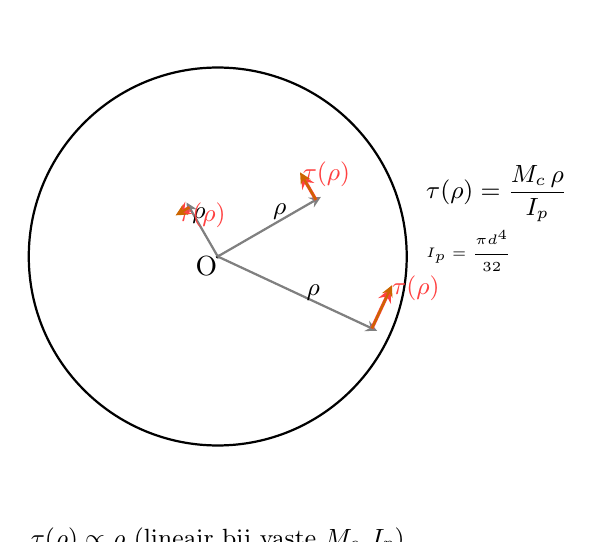
\begin{tikzpicture}[scale=1.2,>=stealth,inner sep=0pt]
      \def\R{2.0}
      % Styles
      \tikzset{shaft/.style={thick},
               shear/.style={->,>=stealth,red!75,very thick},
               tangent/.style={->,>=stealth,orange!80!black,thick},
               rho/.style={->,gray,thick,>=stealth}}

      % shaft cross-section
      \draw[shaft] (0,0) circle (\R);
      \fill (0,0) circle (0.6pt) node[below left] {O};

      % sample radii with shear (tangent) arrows and rho arrows
      \foreach \r/\ang in {0.6/120,1.2/30,1.8/-25}{%
        % radius line
        \draw[black!60] (0,0) -- (\ang:\r);
        % small rho arrow (radial measure)
        \draw[rho] (0,0) -- (\ang:{\r+0.06}) node[pos=0.6,above,black]{\small $\rho$};
        % shear vector (tangent) and label
        \draw[shear] (\ang:\r) -- ++({\ang+90}:{0.26*\r}) node[pos=1,right]{\small $\tau(\rho)$};
        % extra thin tangent arrow for style
        \draw[tangent] (\ang:\r) -- ++({\ang+90}:{0.28*\r});
      }

      % Formula box outside the cross-section (right side)
      \node[anchor=west,align=left] at (2.2,0.4) {\small $\displaystyle \tau(\rho)=\dfrac{M_c\,\rho}{I_p}$\\[2pt] \tiny $I_p=\dfrac{\pi d^4}{32}$};

      % Small note below (placed explicitly below the circle)
      \node at (0,-3) {\small $\tau(\rho)\propto\rho$ (lineair bij vaste $M_c,I_p$)};
    \end{tikzpicture}
    \caption{Torsiediagram: schuifspanning $\tau$ neemt lineair toe met de straal $\rho$; relevante formule staat buiten de doorsnede.}
    \label{fig:torsie_cirkel}
  \end{figure}
  Met het traagheidsmoment berekent als volgt (zie statica):
  \newline
\theoriebox{\textbf{Polair traagheidsmoment voor een cirkelvormige doorsnede:} $I_p = \frac{\pi d^4}{32}$}

De combinatie van deze formules:

\frm{Maximale schuifspanning bij Draaien}{M_d = C_b \cdot d^{x_w}}{waarbij \ensuremath{C_b} de schuifspanningcoëfficiënt is,
\ensuremath{d} de diameter, \ensuremath{x_w} de schuifspanningsexponent.}


\frm{Maximale verspanningsmoment}{M_c = a\cdot M_b}{waarbij \ensuremath{M_c} het verspaningsmoment is en \ensuremath{M_b} het maximale verspanningsmoment.}


  Samen met het verspanningsmoment:

  \medskip
  \noindent\textbf{Afleiding van de maximale voeding $f_{\max}$ (twee methodes)}

  \paragraph{1) Via het schuifspanningscriterium}
  De maximale schuifspanning in de buitenvezel van een ronde doorsnede is
  \[
  \tau_{\max}=\dfrac{16\,M_c}{\pi\,d^3}.
  \]
  Eis \(\tau_{\max}\le\tau_{\mathrm{allow}}\):
  \[
  M_c \le \dfrac{\tau_{\mathrm{allow}}\,\pi\,d^3}{16}.
  \]
  Met \(M_c = C_m\,d^{x_M}\,f^{y_M}\) volgt
  \[
  f_{\max} = \left(\dfrac{\tau_{\mathrm{allow}}\,\pi}{16\,C_m}\right)^{1/y_M} d^{(3-x_M)/y_M}.
  \]

  \paragraph{2) Via een momentlimiet}
  Als \(M_c\le M_d=C_b\,d^{x_w}\) dan volgt
  \[
  f_{\max} = \left(\dfrac{C_b}{C_m}\right)^{1/y_M} d^{(x_w-x_M)/y_M}.
  \]

  \paragraph{Speciale geval -- lineair}\hfill\\
  Wanneer \(y_M=1\) en \(x_w-x_M=1\) volgt
  \[
  f_{\max} = \dfrac{C_b}{C_m}\; d,
  \]
  wat overeenkomt met de eenvoudige vorm \(f_{\max}=C\cdot d\).




  \frm{Maximale voeding bij boren}{f_{max} = C \cdot d}{waarbij $C$ een constante is, $d$ de diameter en $f_{max}$ de maximale voeding.}


  \frm{Kracht $F_f$ is de kracht recht naar boven bij een boormachine}{F_f = C_f \cdot d^{X_f} \cdot f^{y_f}}{waarbij $C_f$ de voedingskrachtcoëfficiënt is, $d$ de diameter, $f$ de voeding en $X_f$ en $y_f$ de voedingskrachtsexponenten.}

  Deze kracht zal een moment creeëren op de machine die hem kan buigen. 
  Dit is vooral bij C vormige structuren.

  \begin{figure}[H]
    \centering
    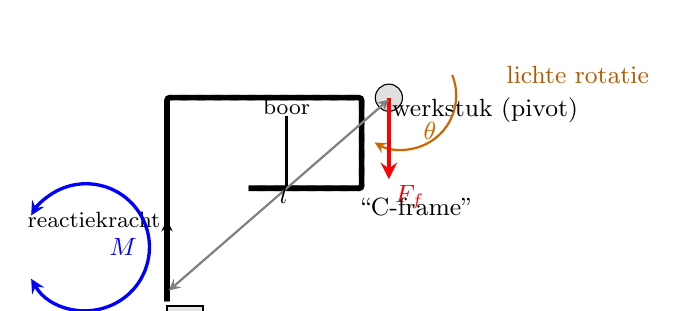
\begin{tikzpicture}[scale=1.15,>=stealth,inner sep=0pt,every node/.style={font=\small}]
      % Styles
      \tikzset{frame/.style={line width=2pt,rounded corners=1pt},
               support/.style={line width=0.8pt,draw=black,fill=black!10},
               spindle/.style={line width=1.2pt},
               load/.style={->,ultra thick,red,>=stealth},
               reaction/.style={->,thick,black},
               moment/.style={<->,very thick,blue,>=stealth},
               dim/.style={<->,thick,gray, >=stealth},
               rotarc/.style={->,thick,orange!80!black,>=stealth}}

      % Coordinates (parameterised for easier tuning)
      \coordinate (A) at (-1.2,-1.0);
      \coordinate (B) at (-1.2,1.25);
      \coordinate (C) at (0.95,1.25);
      \coordinate (D) at (0.95,0.25);
      \coordinate (E) at (-0.3,0.25);

      % Frame (neutral position)
      \draw[frame] (A) -- (B) -- (C) -- (D) -- (E);

      % Base support (stylised)
      \draw[support] ($(A)+(0,-0.15)$) rectangle ($(A)+(0.4,-0.05)$);

      % Workpiece / pivot (drawn as slightly larger disc)
      \coordinate (wp) at (1.25,1.25);
      \filldraw[fill=black!12,draw=black] (wp) circle (0.15cm) node[below right,xshift=1pt]{\small werkstuk (pivot)};

      % Rotated (deformed) frame: small rotation around 'wp' to show the machine tilting
      \draw[frame,dashed,opacity=0.7,rotate around={-8:(wp)}] (A) -- (B) -- (C) -- (D) -- (E);

      % Small rotation arc and label theta (moved slightly to avoid overlap)
      \draw[rotarc] ($(wp)+(0.7,0.25)$) arc (22:-120:0.6) node[midway,left,yshift=2pt]{\small $\theta$};
      \node[orange!70!black,right=8pt] at ($(wp)+(1.05,0.25)$){\small lichte rotatie};

      % Spindle / tool (fixed to the neutral frame)
      \draw[spindle] (0.12,0.25) -- ++(0,0.8) node[above,black]{\footnotesize boor};

      % Feed force applied to the workpiece (axial, pointing downward towards the support)
      \draw[load] (wp) -- ++(0,-0.9) node[below right=2pt]{$F_f$};

      % Reaction arrow at the base (upward, offset to avoid overlap)
      \draw[reaction] ($(A)+(0,0.2)$) -- ++(0,0.7) node[left=2pt,pos=1,black]{\footnotesize reactiekracht};

      % Bending moment arc on the left with arrows both ends (shows moment due to Ff about pivot)
      \draw[moment] ($(A)+(-1.5,0.25)$) arc (-150:150:0.7) node[midway,left,xshift=-4pt]{\small $M$};

      % Dimension (lever arm from left vertical to pivot)
      \draw[dim] ($(wp)+(0,-0.02)$) -- ($(A)+(0.02,0.12)$) node[midway,right,black]{\small $l$};

      % Annotations (moved further down to avoid collision with text)
      \node[below] at ($(C)+(0.6,-1.1)$) {\small ``C‑frame''};
    \end{tikzpicture}
    \caption{C‑vormig frame: axiale voedingskracht $F_f$ op het werkstuk (pivot) veroorzaakt een lichte kanteling (\(\theta\)) rond het werkstuk; de gestippelde lijn toont de gedraaide positie van het frame.}
    \label{fig:Cframe_moment}
  \end{figure}
  \FloatBarrier


  \section{Boormachines en booroperaties in de industrie.}
\subsection{NC-gestuurde boormachines}
NC-gestuurde boormachines (Numerical Control) zijn computergestuurde machines die worden gebruikt voor het boren van gaten in materialen met 
hoge precisie en herhaalbaarheid.
 Deze machines maken gebruik van vooraf geprogrammeerde instructies 
 om de bewegingen van de boor en het werkstuk te regelen.
\newline

\subsection{Boren}
Hier zijn nog relevante type boren en hun toepassingen:
\begin{itemize}
  \item \textbf{Toepassingen:} verspanen van gaten voor bevestigingsmiddelen, passingen en nabewerkingen (ruimen, kotteren); wordt ook gebruikt als pilot voor grotere bewerkingen.
  \item \textbf{Belangrijke parameters:} snijsnelheid $v_c$, voeding $f$, snedediepte $a$, koelmiddel en spanenvorm.
  \item \textbf{Veelvoorkomende borentypes:}
    \begin{itemize}
      \item \textbf{Centerboor / positioneerboor:} korte, stijve boor om een startpunt te maken (voorkomt uitlopen van de boor).
      \item \textbf{Steekboor (jobber / stub):} standaard boor voor algemene gaten; lengte en spiraaltype kiezen afhankelijk van diepte en spanenafvoer.
      \item \textbf{Verzinkingsboor (countersink):} maakt een conische uitsparing voor schroefkoppen of voor ontbraamwerk.
      \item \textbf{Split‑point / conische punt boren:} verbetert centrering en vermindert wander bij start.
    \end{itemize}
\end{itemize}
\begin{figure}[ht]
  \centering
  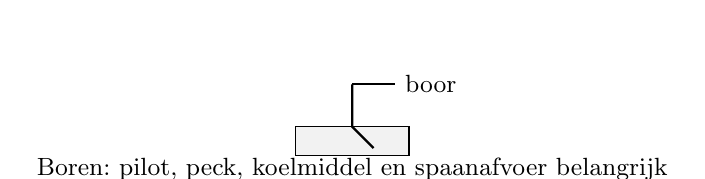
\begin{tikzpicture}[scale=0.9]
    % Simple drill icon
    \draw[fill=gray!10] (-0.8,0) rectangle (0.8,-0.4);
    \draw[thick] (0,0.6) -- (0,0) -- (0.3,-0.3);
    \draw[thick] (0,0.6) -- (0.6,0.6) node[right]{\small boor};
    \node at (0,-0.6){\small Boren: pilot, peck, koelmiddel en spaanafvoer belangrijk};
  \end{tikzpicture}
  \caption{Schematische weergave van een boor in een werkstuk}
\end{figure}
\paragraph{Type boren}
\begin{itemize}
\item \textbf{Verzinkingsboor}: Wordt gebruikt om een conische uitsparing te maken aan het begin van een gat, zodat schroefkoppen gelijk met het 
oppervlak kunnen liggen.
\item \textbf{Centerboor}: Wordt gebruikt om een startpunt te creëren.
\item \textbf{Steekboor}: Wordt gebruikt voor het boren van algemene gaten.
\end{itemize}

\begin{figure}[ht]
  \centering
  \includegraphics[width=0.8\textwidth]{image44.png}
  \caption{Verschillende soorten boren}
\end{figure}

\subsection{Kotteren}
Als je een groot gat hebt en je kunt niet met een boor zo'n groot gat maken, dan kun je kotteren gebruiken.
Je kunt ook eventueel frezen maar dat zie je in het volgende hoofdstuk \ref{chap:Verspanen_Frezen}
Bij kotteren ga je de boor ook nog laten draaien waardoor je een groter oppervlak gaat verspannen.

\subsection{Draadtappen}
Draadtappen is het snijden van interne schroefdraad in een voorgeboord gat.

\begin{table}[ht]
  \centering
  \begin{tabular}{lcc}
    \toprule
    Schroefdraad & Pitch (mm) & Aanbevolen tap‑boring (mm) \\
    \midrule
    M5~$\times$~0.8 & 0.8 & 4.2 \\
    M6~$\times$~1.0 & 1.0 & 5.0 \\
    M8~$\times$~1.25 & 1.25 & 6.75 \\
    M10~$\times$~1.5 & 1.5 & 8.5 \\
    \bottomrule
  \end{tabular}
  \caption{Veelvoorkomende metrische tap‑boringen}
\end{table}
\subsection{Ruimen}
Ruimen is een afwerkingsbewerking om een bestaand gat op nauwkeurige maat en met goede oppervlaktekwaliteit te brengen
Het zorgt ervoor dat je heel precies gaten kunt maken met een goede oppervlaktekwaliteit.
\begin{figure}[ht]
  \centering
  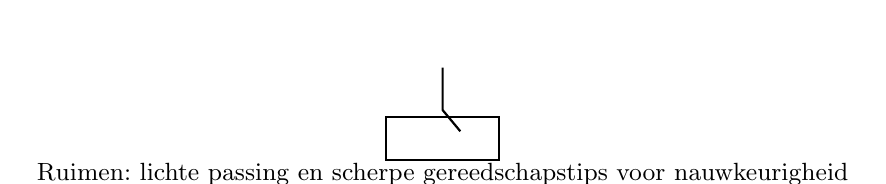
\begin{tikzpicture}[scale=0.9]
    % reamer sketch
    \draw[thick] (-0.8,0) rectangle (0.8,-0.6);
    \draw[thick] (0,0.7) -- (0,0.1) -- (0.25,-0.2);
    \node at (0,-0.8){\small Ruimen: lichte passing en scherpe gereedschapstips voor nauwkeurigheid};
  \end{tikzpicture}
  \caption{Schematische weergave van een reamer in een werkstuk}
\end{figure}


  \chapter{Verspanen: Frezen}
  \label{chap:Verspanen_Frezen}

  Frezen is een verspaningstechniek waarbij een roterend snijgereedschap, de frees, wordt gebruikt om materiaal van een werkstuk te verwijderen.
  Het proces omvat het bewegen van de frees langs het oppervlak van het werkstuk om de gewenste vorm of maat te bereiken.

  \textbf{- hoofdbeweging}
  \newline
  Je gereedschap de \textbf{frees} gaat roteren en het werkstuk kan ook roteren.
  \newline
  \textbf{- voedingsbeweging}
  \newline
  Het gereedschap of het werkstuk gaat bewegen om materiaal te verwijderen.
  \newline

  \section{Inleiding Frezen}

    \textbf{- hoofdbeweging}
  \newline
  Je gereedschap de \textbf{frees} gaat roteren en het werkstuk kan ook roteren.
  \newline
  \textbf{- voedingsbeweging}
  \newline
  Het gereedschap of het werkstuk gaat bewegen om materiaal te verwijderen.
  \newline

  \subsection{Soorten frezen}
  Als je gaat frezen via met de as-richting van de frees in de lengteas van de frees, noem je dit \textbf{mantelfrezen}.
  \newline
  Als je met de punt van de frees gaat frezen noem je dit \textbf{kopfrezen}.

  \subsection{Geometrie van de frees}

  Net zoals bij draaien en boren zijn er verschillende vlakken op de frees die verschillende functies hebben.
  \begin{itemize}
  \item \textbf{Spaangroef}
  \item \textbf{Vrijloophoek}
  \item \textbf{Snijkant}
  \item \textbf{Snijvlak}
  \item \textbf{wighoek}
   \end{itemize}

   Deze hebben dezelfde eigenschappen als bij boren en draaien.
    Je kunt meer info vinden bij Algemeen verspannen~\ref{chap:Algemeen verspanen}.

   \begin{figure}[ht]
    \centering
    \includegraphics[width=0.6\textwidth]{image45.png}
    \caption{Geometrie van een mantelfrees}
    \end{figure}


    \section{krachtwerking bij frezen}

    Net zoals bij draaien en boren zijn er verschillende krachten die op het werkstuk
    en de frees werken tijdens het frezen.
    Ze worden met de theorie van Kienzle berekend.

    \begin{figure}[H]
      \centering
      \includegraphics[width=0.60\textwidth,trim=20 8 14 10,clip]{image46.png}
      \caption{Krachten op een frees}
      \label{fig:frees_krachten}
    \end{figure}
    \FloatBarrier

    {\small
    De krachten op de frees zijn voornamelijk de snijkracht $F_c$ en de voedingskracht $F_f$; de terugdrukkracht $F_p$ is meestal kleiner en minder kritisch. Een goed begrip van deze krachten is essentieel voor het optimaliseren van snijparameters en het waarborgen van gereedschapslevensduur.
    }
    \begin{itemize}
      \item Snijkracht $F_c$: hoofdkracht die het snijproces aandrijft.
      \item Voedingskracht $F_f$: kracht die de voeding van de frees aandrijft.
      \item Terugdrukkracht $F_p$: kracht loodrecht op $F_c$ en $F_f$, meestal kleiner.
    \end{itemize}

    De snededikte is niet constant omdat je frees ronddraait. Voor berekeningen wordt de gemiddelde snededikte gebruikt.
    \newline
    \textbf{BELANGRIJK VOOR EXAMEN}\\
    Je krachten op je frees zijn dus niet constant; zorg dat je dit weet voor het examen. Daarom nemen we het gemiddelde snededikte $h_{gem}$ zodat we toch een berekening hebben voor de kracht.

    \theoriebox{\textbf{Gemiddelde snededikte bij Frezen:} $h_{gem} = f_z \cdot \sqrt{\dfrac{a}{d}}$\\\small}
    \newline
    waarbij $f_z$ de voeding per tand is, $a$ de snedediepte en $d$ de diameter van de frees.

    \theoriebox{\textbf{Voeding per tand bij Frezen:} $f_z = \dfrac{f}{z_i}$\\\small}
    \newline
    waarbij $f$ de voeding is en $z_i$ het aantal tanden van de frees.

    \theoriebox{\textbf{Snijsnelheid bij Frezen:} $v_c = \pi \cdot d \cdot n$\\\small}
    \newline
    waarbij $d$ de diameter van de frees is en $n$ het toerental.

    \theoriebox{\textbf{Ingrijpingshoek bij Frezen:} $\displaystyle \phi = \arccos\!\left(1 - \dfrac{2a}{d}\right) \;\Rightarrow\; \cos\phi = \dfrac{2/d \cdot a}{d}$.\\\small}
    \newline
      waarbij $a$ de snedediepte is en $d$ de diameter van de frees.

    \theoriebox{\textbf{Tanden per ingrijping}{$z_i = \frac{Q}{360}\cdot z$}}
    \newline
     waarbij $z_i$ het aantal tanden per ingrijping is,
    $Q$ de ingrijpingshoek in graden en $z$ het totaal aantal tanden van de frees.
    \newline

  \frm{Snijkracht bij Frezen}{\ensuremath{F_c = k_c \cdot b \cdot h_{gem}^{(1-e)} \cdot z_i}}{waarbij $k_c$ de snijkrachtcoëfficiënt is,
  $b$ de snedebreedte, $h_{gem}$ de gemiddelde snededikte, $z_i$ het aantal tanden en $e$ de snijkrachtsexponent.}

  \frm{Snijmoment bij Frezen}{\ensuremath{M_c = C_m \cdot d^{x_M} \cdot f_z^{y_M} \cdot z_i}}{waarbij $C_m$ de momentcoëfficiënt is,
  $d$ de diameter, $f_z$ de voeding per tand, $z_i$ het aantal tanden en $x_M$, $y_M$ de momentexponenten.}

  \frm{Voedingskracht bij Frezen}{\ensuremath{F_f = k_f \cdot b \cdot h_{gem}^{(1-e)} \cdot z_i}}{waarbij $k_f$ de voedingskrachtcoëfficiënt is,
  $b$ de snedebreedte, $h_{gem}$ de gemiddelde snededikte, $z_i$ het aantal tanden en $e$ de voedingskrachtsexponent.}

  Bij frezen zijn de krachten op je freez niet constant.
  De kracht op één tant per draaing is parabolisch en als je de invloed van alle tanden samentelt krijg je een heuvelachtige 
  krachtcurve.
  \begin{figure}[ht]
    \centering
    \includegraphics[width=0.5\textwidth]{47.png}
    \caption{Krachtcurve bij frezen}
    \end{figure}

    \section{Richting van frezen}
    Er zijn twee richtingen van frezen:
    \begin{itemize}
      \item \textbf{Meelopend frezen}: De frees draait in dezelfde richting als de voeding. Dit zorgt voor een betere oppervlaktekwaliteit en minder gereedschapsbelasting.
      \item \textbf{Tegenlopend frezen}: De frees draait in de tegenovergestelde richting van de voeding. Dit kan leiden tot een ruwer oppervlak en hogere gereedschapsbelasting.
    \end{itemize}

    
    \begin{figure}[ht] 
      \centering
      \includegraphics[width=0.8\textwidth]{image48.png}
      \caption{Tegenlopend en meelopend frezen en de krachten die ze creeëren}
      \label{fig:image48.png}
\end{figure}

    \begin{table}[ht]
      \centering
      \caption{Vergelijking: Tegenlopend vs Meelopend frezen}
      \label{tab:meelopend_vs_tegenlopend}
      \small
      \begin{tabular}{p{0.24\textwidth} >{\raggedright\arraybackslash}p{0.36\textwidth} >{\raggedright\arraybackslash}p{0.36\textwidth}}
        \toprule
        \textbf{Kenmerk} & \textbf{Tegenlopend frezen} & \textbf{Meelopend frezen} \\
        \midrule
        \textbf{Aandrijving / voeding} & $F_h$ drukt werkstuk weg van frees. & $F_h$ trekt werkstuk naar frees toe. \\
        \addlinespace
        \textbf{Spelingscompensatie} & Geen compensatie nodig; veiliger bij backlash. & Spelingcompensatie onmisbaar (gevoelig voor backlash). \\
        \addlinespace
        \textbf{Spaanvorming} & Dun $\rightarrow$ dik (chip groeit tijdens snede). & Dik $\rightarrow$ dun (chip neemt af richting einde). \\
        \addlinespace
        \textbf{Snijkracht} & Stijgt geleidelijk tijdens ingreep. & Stijgt sneller; hogere piekbelasting bij ingang. \\
        \addlinespace
        \textbf{Snijgedrag} & Eerst wrijving, later snijden (meer smearing). & Meteen snijden (scherpere insnijding). \\
        \addlinespace
        \textbf{Oppervlaktekwaliteit} & Meestal matig. & Meestal beter (glad). \\
        \addlinespace
        \textbf{Opspanning / stabiliteit} & Neiging tot beurtelende krachten → klapperen / chatter. & Werkstuk wordt 'in klem' getrokken; minder klapperen maar vereist stevige klemmen. \\
        \addlinespace
        \textbf{Nauwkeurigheid} & Kan leiden tot teveel materiaal verwijderd / minder voorspelbaar. & Neiging tot kleinere snij-inhouden (kan preciezer zijn bij goede controle). \\
        \bottomrule
      \end{tabular}
    \end{table}
    \FloatBarrier

    \subsection{Wanneer kiezen: meelopend vs tegenlopend}
    \textbf{Praktische richtlijnen:}
    \begin{itemize}
      \item \textbf{Meelopend (climb milling)} -- kies dit bij een stijve machine en goede opspanning, vooral voor afwerking. De chipdikte neemt af tijdens de ingreep (dik $\rightarrow$ dun), er is minder wrijving bij de instap en doorgaans een betere oppervlaktekwaliteit en langere gereedschapslevensduur; vereist minimale backlash in de aandrijving.
      \item \textbf{Tegenlopend (conventional milling)} -- kies dit bij oudere of minder stijve machines, bij ruwe bewerkingen of wanneer er speling is. De chipdikte neemt toe tijdens de ingreep (dun $\rightarrow$ dik); bij de instap is er meer wrijving en kans op BUE, maar de methode is vaak veiliger voor onstabiele opstellingen of dunwandige onderdelen.
    \end{itemize}

    \paragraph{Effecten op oppervlakte en snedediepte}
    \begin{itemize}
      \item \textbf{Oppervlaktekwaliteit:} Meelopend geeft doorgaans een gladdere afwerking; tegenlopend geeft meer wrijving bij instap en vaak een ruwere afwerking.
      \item \textbf{Snedediepte/productiviteit:} In een stijve opstelling maakt meelopend vaak hogere snededieptes en hogere voedingen mogelijk zonder kwaliteitsverlies; tegenlopend wordt vaak gebruikt voor grove, hoge‑volume snedes of wanneer de machine/opstelling de voorkeur geeft aan een voorzichtige instap.
    \end{itemize}

    \section{Soorten frezen}
    \begin{itemize}
      \item \textbf{Mantelfrezen}: Hierbij wordt de zijkant van de frees gebruikt om materiaal te verwijderen. Dit is geschikt voor het maken van vlakke oppervlakken en contouren.
      \item \textbf{Kopfrezen}: Hierbij wordt de bovenkant van de frees gebruikt om materiaal te verwijderen. Dit is geschikt voor het maken van gaten, sleuven en andere complexe vormen.
      \item \textbf{Bolfrezen}: Hierbij wordt een frees met een bolvormige snijkant gebruikt, geschikt voor het maken van gebogen oppervlakken en complexe 3D-vormen.
      \item \textbf{Vormfrezen}: Hierbij wordt een frees met een specifieke vorm gebruikt om profielen en vormen in het materiaal te frezen.
      \item \textbf{Circulair frezen}: Hierbij wordt een cirkelvormige beweging gebruikt om gaten of cirkelvormige uitsparingen te maken.
      \item \textbf{Trekfrezen of Brootsen}: Hierbij wordt een speciaal gereedschap gebruikt om nauwkeurige vormen en profielen te maken door het materiaal te trekken.
    \end{itemize}

    \section{De Freesmachine}
    Een freezmachine heeft een bank waar je werkstuk wordt op geklemt. Hierop steek je de mantel of kopfreez.
    De freez gaat roteren en de bank gaat bewegen in de x,y en z-richting.


    \begin{figure}[ht] 
      \centering  
      \includegraphics[width=0.8\textwidth]{image49.png}
      \caption{Weergave van een freesmachine}
    \end{figure}


  \chapter{Verspanen:Hybridetechnieken}

  \section{Honen}
  Honen is een slijpoperatie met twee componenten en een heen een weergaande bewegingen.
  \newline
  \textbf{Hoofdbeweging}: Bij honen is de hoofdbeweging een roterende beweging.
  \newline
  \textbf{Voedingsbeweging}: Dit is de beweging waarmee het gereedschap of het 
  werkstuk langzaam wordt verplaatst om het slijpproces voort te zetten.

  Honen helpt met het oppervalktekwaliteit tot en met (IT3)

  \subsection{Lange-slag Honen}

  \subsection{Korte-slag Honen}

  \section{Leppen}

  \section{Hoge snelheid verspanen}

  \section {Laserondersteuning bij verspanen}

  \section{Draadvonken en slijpen}

  \section{ECM (Electro Chemical Machining) en slijpen}





  \chapter{Verspanen:Slijpen}

  Slijpen is een verspaningstechniek waarbij een roterend schijfvormig gereedschap,
   de slijpschijf, wordt gebruikt om materiaal van een werkstuk te verwijderen.
   Verspannen gebeurt door een slijpsteen die kleine deeltjes materiaal \textbf{Snijkorrels} van het werkstuk afneemt.
   Dit oppervlakte is onbepaald en dus is de geometrie niet gekent.
  \newline
   De snijkorrels kunnen oftewel vrij liggen of gebonden zijn in een matrix.
   \newline
   \textbf{Vrije snijkorrels:} losse korrels die losjes op het werkstuk inwerken of in suspensie of pasta. Voorbeelden: 
    \begin{itemize}
      \item \textbf{Leppen}: korrels in een pasta om zeer nauwkeurige oppervlakken te verkrijgen.
      \item \textbf{Stralen}: korrels in een straal om vuil of roest te verwijderen.
    \end{itemize}
    Je kunt dus korrels door het werkstuk sturen om het oppervlaktekwaliteit te verbeteren.
    \newline 
    Korrel kunnen ook gebonden zijn in een matrix.
    \newline
    \textbf{Gebonden snijkorrels:} korrels die vastzitten in een matrixmateriaal. Voorbeelden:
    \begin{itemize}
      \item \textbf{Slijpschijven}: korrels gebonden in een harde matrix voor het slijpen van metalen.
      \item \textbf{Schuurpapier}: korrels gebonden op papier of stof voor handmatig schuren.
      \item \textbf{Honen}: korrels gebonden in een zachte matrix voor het verbeteren van de oppervlakteafwerking en nauwkeurigheid van gaten.
    \end{itemize}


    \subsection{Frezen met onbepaalde snijkanten}
    Bij slijpen heb je een grote negatieve \textbf{Spaanhoek} wat het moeilijker maakt om te verspannen.
    De krachtwerking is dus veel hoger. Maar je \textbf{Snedediepte} is veel kleiner dus die combenseren elkaar.

    Een slijpsteen kun je defineren als een frees met onbepaalde snijkanten.
    \newline
  
    \begin{figure}[ht]
        \centering
        \includegraphics[width=0.8\textwidth]{image50.png}
        \caption{Spaanvorming bij slijpen}
        \label{Spaanvorming bij slijpen}
    \end{figure}

    De korrel hier heeft een enorm negatieve spaanhoek. De spaanvorming is enorm klein maar omdat de korrels 
    zo klein en hard zijn kun je zelfs heel harde materialen slijpen.
    \newline
    \subsection{Eigenschappen van slijpen}
    \begin{enumerate}
      \item \textbf{Snijsnelheid $v_c$}: De snelheid is ongeveer 25 tot 60 m/s, Heel hoge snelheden.
      \item \textbf{Krachten $F_c$}: De krachten zijn hoog door de negatieve spaanhoek en omdat je harde materialen kunt slijpen.
      \item \textbf{Warmteontwikkeling}: Veel energie gaat verloren als warmte, slijpen kan aan het oppervlakte een temperatuur van \textbf{800 tot 900°C} veroorzaken.
      Dit kan leiden tot thermische beschadiging van het werkstuk. Je hebt dus materiaalveranderingen aan het oppervlakte. 
      Intensieve koeling is dus nodig.
      \item \textbf{Snedediepte $a$}: Zeer kleine snededieptes, typisch in de orde van micrometers.
      \item \textbf{Slijtage van de slijpkorrel}: Slijpkorrels worden bot en vallen er dan af.
       Je moet de slijpschijf dus regelmatig vernieuwen of terug op maat brengen. Je neemt dan een stuk van het oppervlakte af. 
      Dit noemt(dressing).
      \item \textbf{Oppervlaktekwaliteit}: Slijpen kan zeer fijne oppervlakteafwerkingen bereiken, vaak in de orde van enkele micrometers $R_a$.
      \item \textbf{Nauwkeurigheid}: Slijpen gaat op machine die enorm stevig zijn en dus niet veel bewegen tijdens het slijpen. 
      Hierdoor kun je zeer nauwkeurige afmetingen bereiken.
      \item \textbf{Toepassingen}: Slijpen kan toegapast worden op zelfs zeer harde materialen zoals gehard staal, keramiek en zelfs diamant.
    \end{enumerate}

    \subsection{Parameters slijpsteen}

    \begin{itemize}
      \item \textbf{Korrelgrootte}: Grotere korrels 
      verwijderen materiaal sneller maar geven een ruwere afwerking; kleinere korrels geven een fijnere afwerking.
      \item korrelgrote 
      \item \textbf{Bindmiddel}: Het materiaal dat de korrels bij elkaar houdt, beïnvloedt de slijpsteen's hardheid en duurzaamheid.
      \item Hardheid van de slijpsteen: Hardere slijpstenen zijn duurzamer maar kunnen ook sneller de korrels verliezen.
      \item Structuur
    \end{itemize}

    \begin{figure}[ht]
      \centering
      \includegraphics[width=0.8\textwidth]{image51.png}
      \caption{Doorsnede van een slijpschijf}
      \label{fig:slijpsteen doorsnede.png}
    \end{figure}
    \subsubsection{Korrelmateriaal}
    \textbf{Natuurlijke korrels} zijn kwarts, korundum en diamant.
    \newline
    \textbf{Kunstmatige korrels} zijn siliciumcarbide en aluminiumoxide.
    \newline
    \subsubsection{Korrelgroot}
    De korrelgrootte bepaald hoeveel je kunt afnemen.
    Grote korrels -> meer afnemen maar je oppervlaktekwaliteit is slechter.
    Kleine korrels -> minder afnemen maar je oppervlaktekwaliteit is beter.
    \newline
    Korrelgrootte wordt aangegeven door mazen per $\text{inch}^2$.

    \subsubsection{Hardheid van de slijpsteen}
    De hardheid is de sterkte van de korrels. 
    De slijpverhouding $G$ = $\frac{\text{volume verspaand materiaal}}{\text{volume slijpschijf per tijdseenheid}}$.
    Een grote $G$ kan je veel materiaal afnemen tegenover hoeveel slijpschijf je verliest.
    \newline
    een kleine $G$ betekent dat je veel slijpschijf verliest tegenover hoeveel materiaal je afneemt.
    \newline
    Je kunt geen hard materiaal slijpen met een zachte slijpsteen omdat de korrels dan te snel bot worden.
    \subsubsection{Bindmiddel}
    Het bindmiddel houdt de korrels bij elkaar.
    een paar voorbeelden zijn keramisch klei, mineralen, metaal en elastische materialen.
    \newline
    \theoriebox{Bijvoorbeeld bij pasta slijpen word een elastisch bindmiddel zodat de korrels overal op het werkstuk kunnen bewegen. We spreken dan niet van een slijpverhouding $G$ omdat die niet relevant is}

\subsubsection{Structuur}
De grote van de porien in verhouding tot het volumeaandeel bindmiddel en korrels.
\newline
Die porien zijn belangrijk. Die zijn kleine openingen tussen de korrels. 
Stukjes spaan gaan in die porien. De poriegrootte moet je aanpassen afhankelijk van de operatie en het contacttijd van de slijpschijf op het werkstuk. 
\newline

Met al deze dingen kunnne een slijpsteen karateriseren.

\textbf{WETEN DAT AL DEZE DIINGEN EEN SLIJPSTEEN KARATERISEREN}

\begin{figure}[ht]
      \centering
      \includegraphics[width=0.8\textwidth]{image52.png}
      \caption{}
      \label{fig:karateriseren van slijpsteen.png}
\end{figure}

\section{temperaturen bij slijpen}

$70 percent$ van de energie die je inbrengt bij het slijpen gaat verloren als warmte.
dit kan leiden tot thermische beschadiging van het werkstuk.
Je moet oppassen voor 
\begin{itemize}
  \item \textbf{Vonken}
  \item \textbf{Structuurveranderingen}
  \item \textbf{Verbranding}
  \item \textbf{Scheurtjes}
  \item \textbf{Residuële spanningen}
\end{itemize}

Je moet dus voldoende koelen of nog een laatste warmtebehandeling doen na het slijpen.
\begin{figure}[ht]
   \centering
   \includegraphics[width=0.8\textwidth]{image53.png}
   \caption{Warmte bij Slijpen}
   \label{fig:warmte_bij_slijpen.png}
\end{figure}

\section{Slijptechnieken}

\begin{figure}[ht]
  \centering
  \includegraphics[width=0.8\textwidth]{image54.png}
  \caption{Alle soorten slijptechnieken}
  \label{fig:Slijptechnieken.png}
\end{figure}

Profielslijpen is slijpen van een bepaald profiel. Je slijpsteen heeft dus een gewenste vorm,
waar je het werkstuk mee slijpt.
\newline

\textit{Tip, is hij niet veel op ingegaan.}


\section{De slijpmachine}
Slijpmachines zijn enorm stijve machines omdat je enorm 
je snedediepte enorm klein is kan kleine bewegingen ervoor zorgen dat je ineens niet meer slijpt. 
Je moet dus in orde van micrometer werken.

\subsection{Centerloos slijpen}
Centerloos slijpen is een slijptechniek waarbij het werkstuk niet wordt vastgehouden door een as of klem, maar in plaats daarvan wordt ondersteund door twee rollen en aangedreven door een derde rol.
\begin{figure}[ht]
   \centering
     \includegraphics[width=0.8\textwidth]{image55.png}
     \caption{Centerloos slijpen}
     \label{fig:centerloos_slijpen.png}
\end{figure}

\subsection{Profielslijpen}
Zoals hiervoor gezegt. Je slijpt een bepaald profiel met een slijpsteen die dat profiel heeft.

  \chapter{Fysische en Chemische afnemende bewerkingen}

  \chapter{Scheiden}
  \chapter{Automatiseren \& machinekeuze}

  \chapter{Productie werkvoorbereiding}


  \chapter{Productiegericht ontwerpen}





\end{document}